\documentclass[
11pt,
a4paper,
pdftex,
czech,
titlepage
]{report}

\usepackage[czech]{babel}
\usepackage[utf8]{inputenc}
\usepackage{lmodern}
\usepackage{textcomp}
\usepackage[T1]{fontenc}
\usepackage{amsfonts}
\usepackage{titlesec}
\usepackage{graphicx}
\usepackage[pdftex]{hyperref}
\usepackage[a4paper,left=30mm,right=30mm,top=28mm,bottom=30mm]{geometry}
\usepackage{enumitem}
\usepackage[final]{pdfpages}
\usepackage{listings}
\hypersetup{colorlinks=true,
  unicode=true,
  linkcolor=black,
  citecolor=black,
  urlcolor=black,
  bookmarksopen=true}

\titleformat{\chapter}
  {\normalfont\LARGE\bfseries}{\thechapter}{1em}{}
\titlespacing*{\chapter}{0pt}{0ex plus 1ex minus .2ex}{2.0ex plus .2ex}

\begin{document}

\begin{titlepage}
	%\vspace*{-2cm}
	{\centering
\includegraphics[scale=1.2]{img/logo-FAV.pdf}\par}
	\centering
	\vspace*{2.5cm}
	{\Large Semestrální práce z KIV/IR\par}
	\vspace{1.5cm}
	{\Huge\bfseries Implementace vlastního systému automatické indexace a vyhledávání dokumentů\par}
	\vspace{2.5cm}

	{\Large Zdeněk Častorál\par}
	{\Large A19N0026P\par}
	{\Large zcastora@students.zcu.cz\par}

	\vfill

	{\Large 30.\,5.\,2020}
\end{titlepage}

\tableofcontents
\thispagestyle{empty}
\clearpage

\newpage
\chapter{Zadání}\label{zadani}
\setcounter{page}{3}
Cílem semestrální práce je implementovat komplexní systém automatické indexace a vyhledávání dokumentů s využitím hotových knihoven pro preprocessing.

Systém po předchozím předzpracování zaindexuje zadané dokumenty a poté umožní vyhledávání nad vytvořeným indexem. Vyhledávání je možné zadáním dotazu s logickými operátory AND, OR, NOT a s použitím závorek. Výsledek dotazu by měl vrátit top x (např. 10) relevantních dokumentů seřazených dle relevance.

Semestrální práce se bude testovat indexací dokumentů a vyhledáváním relevantních dokumentů nad vytvořeným indexem. K~evaluaci bude použit evaluační skript, proto je nutné, aby projekt obsahoval třídy z projektu Interface.

Semestrální práce musí umožňovat zaindexování poskytnutých dat a dat stažených na~cvičení (1. cvičení Crawler).

\section{Minimální nutná funkčnost}\label{min_func}
Implementace semestrální práce musí nutně obsahovat:
\begin{itemize}
    \item tokenizaci,
    \item preprocessing (stopwords remover, stemmer/lemmatizer),
    \item vytvoření in-memory invertovaného indexu,
    \item tf-idf model,
    \item cosine similarity,
    \item vyhledávání pomocí dotazu (top x výsledků seřazených dle relevance),
    \item vyhledávání s pomocí logických operátorů AND, OR, NOT,
    \item podporu závorek pro vynucení priority operátorů.
\end{itemize}

\section{Nadstandardní funkčnost}\label{adv_func}
Nadstandardní funkčnosti semestrální práce jsou například:
\begin{itemize}
    \item file-based index,
    \item pozdější doindexování dat (přidání nových dat do existujícího indexu),
    \item ošetření např. HTML tagů,
    \item detekce jazyka dotazu a indexovaných dokumentů,
    \item vylepšení vyhledávání,
    \item vyhledávání frází,
    \item vyhledávání v okolí slova,
    \item více scoring modelů,
    \item indexování webového obsahu,
    \item další předzpracování normalizace,
    \item GUI/webové rozhraní,
    \item napovídání keywords,
    \item podpora více polí pro dokument,
    \item CRUD indexovaných dokumentů,
    \item zvýraznění hledaného textu v náhledu výsledků,
    \item dokumentace psaná v TEXu,
    \item implementace dalšího modelu (použití sémantických prostorů).
\end{itemize}


\chapter{Analýza}
V~rámci analýzy byla aplikace rozdělena na následující hlavní části:
\begin{itemize}
    \item předzpracování (preprocessing),
    \item vytvoření invertovaného indexu (zaindexování dokumentů),
    \item booleovské vyhledávání,
    \item vektorové vyhledávání,
    \item příkazový interpret.
\end{itemize}

\section{Předzpracování (preprocessing)}\label{analyza_preprocess}
Před samotnou indexací dokumentu je nutné jej předzpracovat. Na kvalitě předzpracování závisí celková kvalita vyhledávání. Předzpracování obecně obsahuje následující hlavní části:

\begin{itemize}
    \item tokenizace -- rozdělení vstupu na jednotlivé tokeny,
    \item vyjmutí stop slov -- odstranění předem definovaných slov,
    \item stemming a lematizace -- převedení slov do jejich základního tvaru nebo jejich kořenu.
\end{itemize}


\section{Invertovaný index}\label{inv_index_analyza}
Invertovaný index je datová struktura používaná pro fulltextové vyhledávání v rozsáhlých kolekcích dokumentů. Obvykle se jedná o seřazenou kolekci předzpracovaných slov, kde ke~každému slovu (resp. termu) je přiřazen seznam dokumentů, ve kterých se slovo vyskytuje.

V~rámci každé položky v seznamu dokumentů v invertovaném indexu jsou uchovávány další informace: 
\begin{itemize}
    \item \texttt{\textbf{documentId}} -- identifikátor dokumentu,
    \item \texttt{\textbf{count}} -- počet opakování daného slova v příslušném dokumentu (TF - term frequency),
    \item \texttt{\textbf{tfidf}} -- složka TF-IDF odpovídající danému slovu v invertovaném indexu pro daný dokument (\texttt{documentId}).
\end{itemize}

Položka v seznamu dokumentů je reprezentována třídou \texttt{DocInfo} (viz obrázek \ref{docInfo_analyza}).

\begin{figure}[!ht]
	\centering
	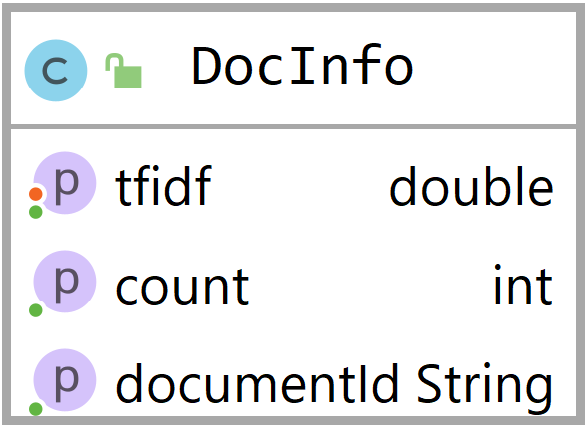
\includegraphics[scale=0.25]{img/DocInfo.png}
	\caption{Položka \texttt{DocInfo} v invertovaném indexu}
	\label{docInfo_analyza}
\end{figure}

\subsection{Reprezentace invertovaného indexu}
Invertovaný index lze realizovat dvěma základními variantami:
\begin{itemize}
    \item \textit{maticí},
    \item \textit{spojovou strukturou (mapou)}.
\end{itemize}

První variantou je realizace invertovaného indexu prostřednictvím \textit{matice} o rozměrech $|T|\times|D|$, kde $T$ je množina termů a $D$ je množina dokumentů. Pro každý term je v matici uložen seznam položka \texttt{DocInfo} pro každý dokument. Toto řešení je značně neekonomické, jelikož je nutné alokovat paměť pro celý rozsah matice, tzn. i pro dokumenty, které daný term neobsahují. 

Vhodnějším řešením je použít spojovou strukturu či mapu, kde pro každý term jsou ukládány pouze ty dokumenty, ve kterých se daný term vyskytuje. Toto řešení zabírá podstatně méně paměti než předchozí řešení a také vyhledávání je rychlejší (vzhledem k~tomu, že nemusíme procházet celou matici). V~rámci této semestrální práce byla použita \textit{mapa}, kde \textit{klíčem} je daný term a \textit{hodnotou} je další mapa, jejíž \textit{klíčem} je identifikátor dokumentu a \textit{hodnotou} položka \texttt{DocInfo} (viz obrázek \ref{inv_index_analyza}). Tato struktura byla použita z důvodu rychlejšího prohledávání v položkách pro daný term, oproti použití spojového seznamu.

\begin{figure}[!ht]
	\centering
	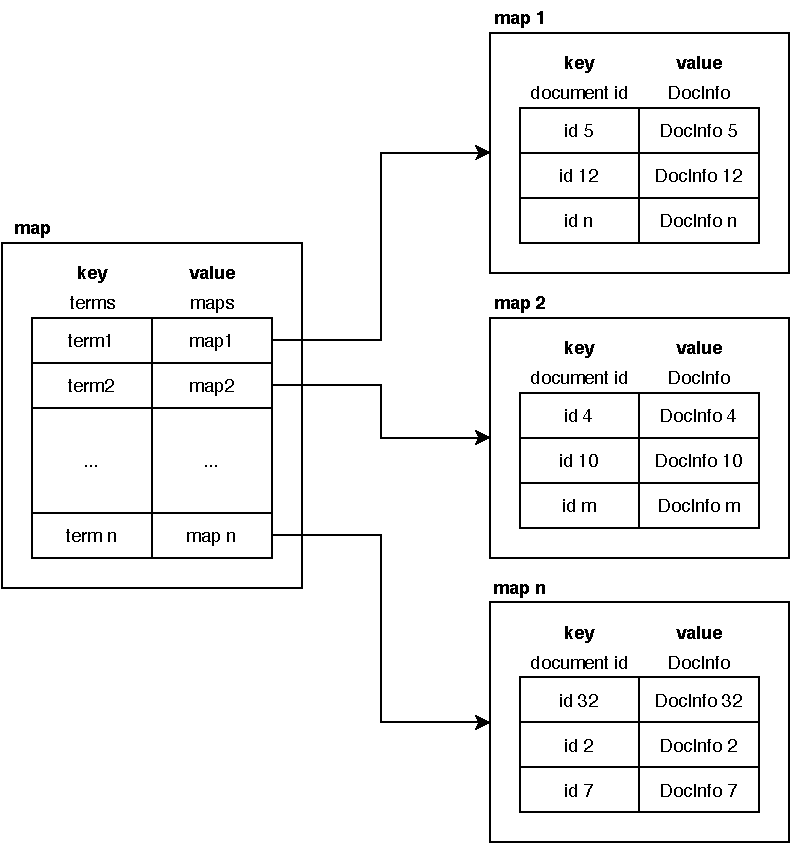
\includegraphics[scale=0.93]{img/invertedIndex.pdf}
	\caption{Realizace invertovaného indexu}
	\label{inv_index_analyza}
\end{figure}

\section{Vektorový model vyhledávání}
V~rámci semestrální práce byl realizován \textit{vektorový model vyhledávání}. Jedná se o~implementaci ohodnoceného vyhledávání, kde každému dokumentu je přiřazeno skóre relevance k danému dotazu. Dokumenty jsou poté seřazeny dle tohoto skóre sestupně.

Každý dokument je reprezentován vektorem $\vec{d_i} = (d_{i1}, d_{i2}, ..., d_{im})$ reálných čísel v~$m$-dimenzionálním prostoru, tzn. $\vec{d_i}\in R^{m}$, kde $i$ je identifikátor dokumentu. Proměnná $m = |V|$, kde $V$ je slovník kolekce dokumentů, každá složka $d_{ij}$ vektoru reprezentuje váhu $j$-tého slova v~$i$-tém dokumentu. Dotaz je také dokument, tzn. lze jej reprezentovat odpovídajícím vektorem.

Nejprve je nutné vypočítat vektory pro dokumenty, včetně dotazu (viz kapitola \ref{analyza_vypocet_vekt}), poté je nutné tyto vektory porovnat, tzn. zjistit jejich podobnost. Čím je podobnost dokumentu s dotazem vyšší, tím je dokument k~danému dotazu relevantnější. Jednou z možností porovnání vektorů je použití \textit{kosinové podobnosti} (viz kapitola \ref{analyza_kosin}).

\subsection{Výpočet vektorů}\label{analyza_vypocet_vekt}
Nejprve je nutné vypočítat \textit{weighted term frequency} (vážená frekvence termu) v daném dokumentu. \textit{Term frequency} (frekvence termu) $tf_{t,d}$ termu $t$ v~dokumentu $d$ označuje, kolikrát se term $t$ vyskytl v~dokumentu $d$. \textit{Weighted term frequency} je možné vypočítat podle následujícího vzorce:

$$wf_{t,d}=1+\log tf_{t,d}$$

\noindent pro $tf_{t,d}>0$, jinak $wf_{t,d}=0$. Tato hodnota udává důležitost termu v dokumentu.

Poté je nutné vypočítat tzv. \textit{inverse document frequency} k~zohlednění důležitosti termu v celé kolekci. \textit{Document frequency} $df_{t}$ termu $t$ označuje počet dokumentů v celé kolekci, ve kterých se term $t$ vyskytl. \textit{Inverse document frequency} se vypočítá následovně:

$$idf_t=\log \frac{N}{df_t},$$
kde $N$ je celkový počet dokumentů v kolekci. Čím více se term $t$ v dokumentech vyskytl, tím bude jeho $idf_t$ nižší. Tato hodnota udává důležitost termu v celé kolekci.

Vynásobením $wf_{t,d}$ váhy a $idf_t$ váhy získáme \textit{tf-idf váhu} $w_{t,d}$ termu $t$ v dokumentu $d$. Tyto váhy jsou poté jednotlivými složkami vektorů dokumentů.

\subsection{Kosinová podobnost}\label{analyza_kosin}
Mějme dotaz, který je popsán vektorem $\vec{q}$ a dokument, který je popsán vektorem $\vec{d}$. Kosinová podobnost pro tyto dva vektory se vypočítá podle následujícího vzorce:

$$\cos(\vec{q},\vec{d})=\frac{\vec{q} \cdot \vec{d}}{||\vec{q}|| \cdot ||\vec{d}||}=\frac{\sum_{i=1}^{m} q_i d_i}{\sqrt{\sum_{i=1}^{m} q_{i}^2} \sqrt{\sum_{i=1}^{m} d_{i}^2}},$$
\noindent kde 
\begin{itemize}
    \item $q_i$ je \textit{tf-idf} váha termu $i$ v dotazu $q$,
    \item $d_i$ je \textit{tf-idf} váha termu $i$ v dokumentu $d$.
\end{itemize}

\section{Booleovský model vyhledávání}
Součástí této semestrální práce je také \textit{booleovský model vyhledávání}. Získané dokumenty s~použitím tohoto modelu jsou \textit{neohodnocené} (slovo se v dokumentu vyskytlo nebo ne). Vyhledávání prostřednictvím tohoto modelu umožňuje použití operátorů \texttt{AND}, \texttt{OR}, \texttt{NOT} a~vynucení priority těchto operátorů pomocí závorek.

Dotazy s využitím logických operátorů musí být v této aplikaci zadávány v \textit{infixové notaci} (operand operátor operand). Parsování tohoto typu dotazu je realizováno s využitím knihovny \textit{Apache Lucene}. Ta se stará o~převod dotazu do~\textit{prefixové notace} (operátor operand operand) a~tento dotaz vrací jako instanci třídy \texttt{Query}. Následně je rekurzivně z~tohoto dotazu vytvořen strom, kde každý z~listů odpovídá termu a~jeho rodičem je booleovský operátor. Pro každý z~listů je získán seznam instancí \texttt{DocInfo} a~podle booleovského operátoru, který je společným rodičem daných uzlů, je proveden buď průnik (operátor \texttt{AND}), sjednocení (operátor \texttt{OR}), nebo doplněk (operátor \texttt{NOT}) daných seznamů. Takto se~postupuje od listů až ke~kořeni stromu, kde je poté uložen výsledek dotazu jako seznam instancí \texttt{DocInfo}.


\chapter{Implementace}
Aplikace byla implementována v~jazyce \texttt{Java} verze \texttt{11} s~využitím knihovny \texttt{Apache Lucene} pro parsování dotazu s~logickými operátory. Jedná se o~konzolovou aplikaci.

\section{Struktura aplikace}
Aplikace je rozdělena do balíků (\texttt{package}) a tříd (\texttt{class}). Hlavní balíky a třídy aplikace jsou:

\begin{itemize}
    \item balík \texttt{counter} -- obsahuje třídy k~výpočtu hodnot TF-IDF a skóre dokumentů při použití vektorového modelu vyhledávání,
    \item balík \texttt{data} -- obsahuje třídy s~potřebnými daty,
    \item balík \texttt{preprocessing} -- obsahuje třídy zajišťující předzpracování dokumentů,
    \item balík \texttt{search} -- obsahuje třídy pro vyhledávání v~dokumentech,
    \item balík \texttt{utils} -- obsahuje pomocné třídy (např. pro vstupy ze souborů a výstupy do~souborů),
    \item třída \texttt{App} -- hlavní třída programu, obsahuje spustitelný bod aplikace,
    \item třída \texttt{Index} -- třída reprezentující index,
    \item třída \texttt{Shell} -- třída sloužící jako příkazový interpret.
\end{itemize}

\section{Předzpracování (preprocessing)}
Předzpracování bylo implementováno v~souladu s~analýzou uvedenou v~kapitole \ref{analyza_preprocess}. Na~obrázku \ref{uml_preprocess} je uveden UML diagram balíku \texttt{preprocessing}. Předzpracování je možno nakonfigurovat podle potřeb. Ve třídě \texttt{Index} se vytváří instance třídy \texttt{BasicPreprocessing}, kde je možné prostřednictvím parametrů zvolit konfiguraci předzpracování.

\begin{figure}[!ht]
	\centering
	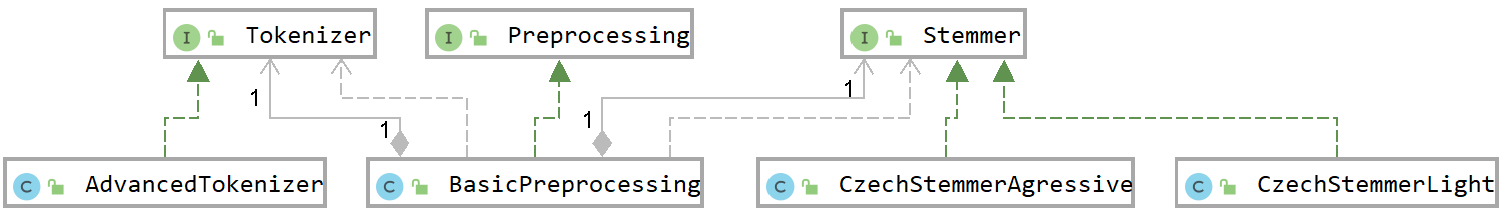
\includegraphics[width=1\textwidth]{img/preprocessing.png}
	\caption{UML diagram balíku \texttt{preprocessing}}
	\label{uml_preprocess}
\end{figure}

\section{Indexace dokumentů}
Dokumenty jsou ukládány do invertovaného indexu, který je reprezentován mapou (viz kapitola \ref{inv_index_analyza}). Konkrétně je použita třída \texttt{HashMap<T>}, která používá \textit{hashování} klíčů, díky kterému má vyhledávání podle klíče v~této mapě složitost $O(1)$. 

V~rámci šetření paměti jsou v mapě ukládány pro každý term pouze ty dokumenty, které daný term obsahují. Vyšší rychlosti vyhledávání je dosaženo předpočítáváním hodnot TF-IDF jednotlivých dokumentů pro dané termy již při indexaci dokumentů. Vektor $idf$ je rovněž vypočítán již při indexaci, stejně jako \textit{normy} (velikosti) vektorů jednotlivých dokumentů. Na obrázcích \ref{uml_indexing1}, \ref{uml_indexing2} a \ref{uml_indexing3} jsou uvedeny UML diagramy tříd zabývajících se indexováním dokumentů.

\begin{figure}[!ht]
	\centering
	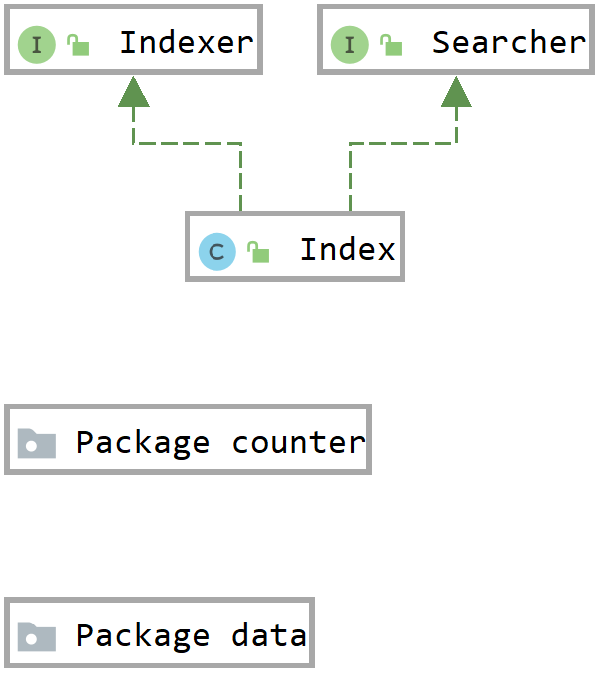
\includegraphics[scale=0.35]{img/indexing1.png}
	\caption{UML diagram -- indexování}
	\label{uml_indexing1}
\end{figure}

\begin{figure}[!ht]
	\centering
	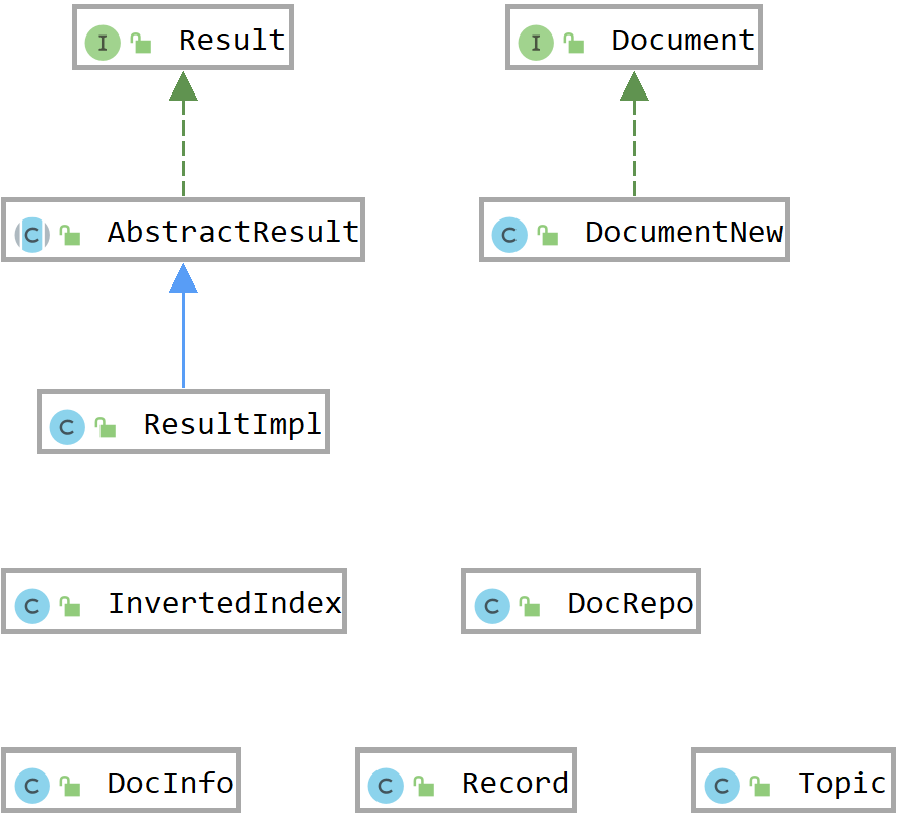
\includegraphics[scale=0.35]{img/indexing2.png}
	\caption{UML diagram -- indexování (package \texttt{data})}
	\label{uml_indexing2}
\end{figure}

\begin{figure}[!ht]
	\centering
	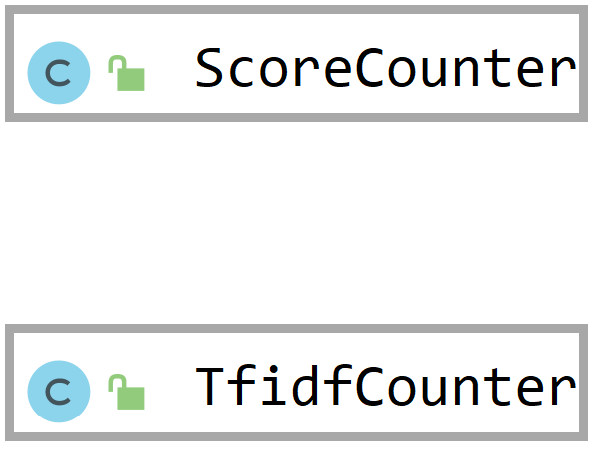
\includegraphics[scale=0.20]{img/indexing3.png}
	\caption{UML diagram -- indexování (package \texttt{counter})}
	\label{uml_indexing3}
\end{figure}

\section{Vyhledávání v dokumentech}
Aplikace umožňuje jak ohodnocené vyhledávání pomocí \textit{vektorového modelu}, tak neohodnocené vyhledávání pomocí \textit{booleovského modelu}. Při vyhledávání prostřednictvím booleovského modelu je možné použít logické operátory \texttt{AND}, \texttt{OR}, \texttt{NOT} a vynutit prioritu operátorů pomocí závorek. Booleovský dotaz musí být v~aplikaci zadán v~\textit{infixové notaci} (operand operátor operand). Při ohodnoceném vyhledávání je výpočet kosinové podobnosti dokumentu s~dotazem prováděn pouze pro dokumenty, které obsahují daný term z~dotazu. Díky tomu je vyhledávání rychlejší a je ušetřena paměť, oproti variantě počítání kosinové podobnosti všech dokumentů s dotazem. UML diagramy tříd zabývajících se vyhledáváním jsou uvedeny na obrázcích \ref{searching1} a \ref{searching2}.

\begin{figure}[!ht]
	\centering
	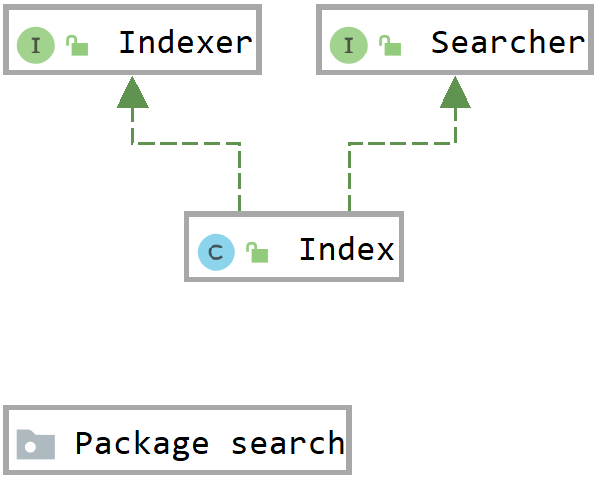
\includegraphics[scale=0.30]{img/searching1.png}
	\caption{UML diagram -- vyhledávání (package \texttt{counter})}
	\label{searching1}
\end{figure}

\begin{figure}[!ht]
	\centering
	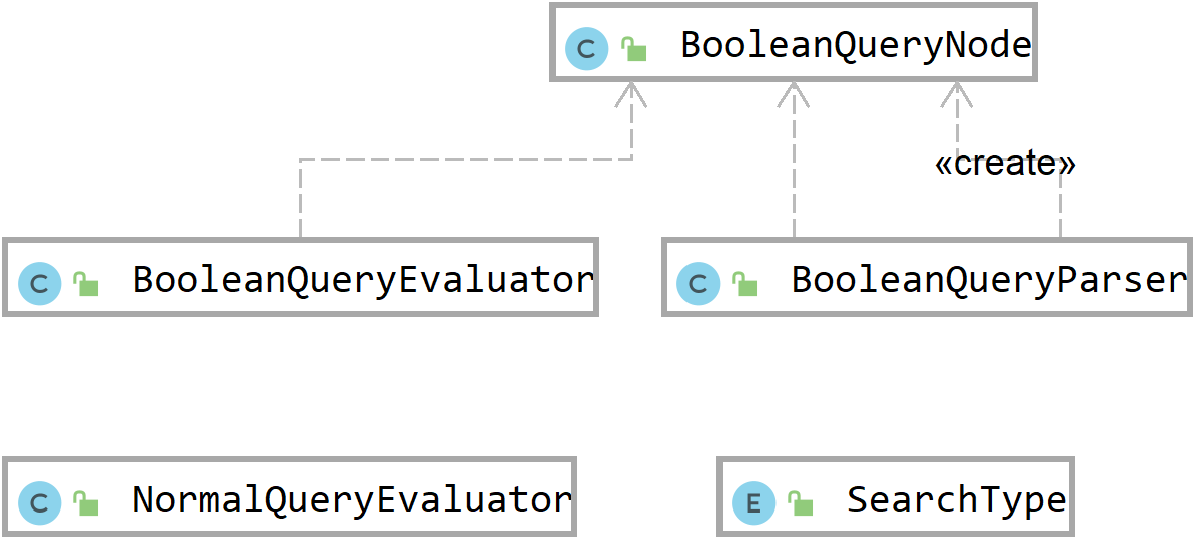
\includegraphics[scale=0.30]{img/searching2.png}
	\caption{UML diagram -- vyhledávání (package \texttt{search})}
	\label{searching2}
\end{figure}

\section{Nadstandardní rozšíření}
V rámci semestrální práce byly realizovány následující nadstrandardní rozšíření:
\begin{itemize}
    \item \textit{file-based index} -- index je možné uložit do souboru a následně jej z tohoto souboru načíst,
    \item \textit{pozdější doindexování dat} -- do existujícího indexu, který již obsahuje množinu dokumentů, je možné zaindexovat další množinu dokumentů,
    \item \textit{CRUD indexovaných dokumentů} -- aplikace umožňuje vytvořit nový dokument a~následně jej zaindexovat, upravit existující dokument v~indexu a~odstranit dokument z~indexu,
    \item \textit{dokumentace psaná v TEXu}.
\end{itemize}


\chapter{Uživatelská příručka}
V této kapitole je popsáno spuštění a ovládání aplikace. 

\section{Spuštění aplikace}
Pro spuštění aplikace je nutné mít nainstalované \texttt{JRE} alespoň verze \texttt{8}. Po~spuštění aplikace se v~konzoli vypíše nápověda k~použití aplikace, kde je zobrazen výčet všech příkazů (viz obrázek \ref{uziv_spusteni}). 

\begin{figure}[!ht]
	\centering
	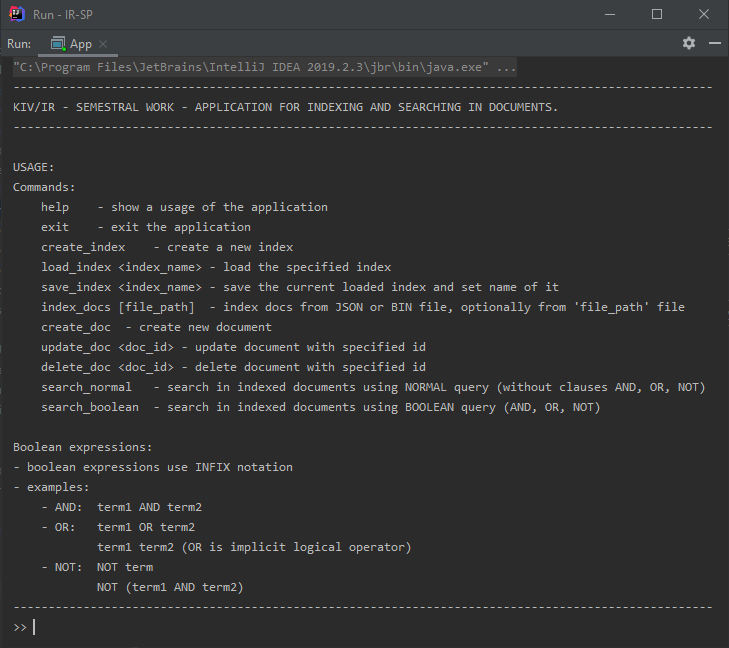
\includegraphics[width=1\textwidth]{img/spusteni.png}
	\caption{Spuštění aplikace}
	\label{uziv_spusteni}
\end{figure}
\newpage
\section{Ovládání aplikace}
Aplikace je konzolová, ovládá se přes příkazovou řádku. Příkazy, které lze v aplikaci použít, jsou:

\begin{itemize}
    \item \texttt{help} -- zobrazí nápovědu k použití aplikace,
    \item \texttt{exit} -- ukončí aplikaci,
    \item \texttt{create\_index} -- vytvoří nový index,
    \item \texttt{load\_index <\textit{název indexu}>} -- načte index ze souboru,
    \item \texttt{save\_index <\textit{název indexu}>} -- uloží index do souboru,
    \item \begin{sloppypar}\texttt{index\_docs [\textit{cesta k indexu}]} -- zaindexuje dokumenty z JSON nebo BIN souboru (pokud nebude zadána cesta k~indexu, použije defaultní cestu \texttt{./data/my\_testing\_data.json}),\end{sloppypar}
    \item \texttt{create\_doc} -- vytvoří nový dokument,
    \item \texttt{update\_doc <\textit{id dokumentu}>} -- upraví existující dokument specifikovaný zadaným id,
    \item \texttt{delete\_doc <\textit{id dokumentu}>} -- odstraní dokument z indexu specifikovaný zadaným id,
    \item \texttt{search\_normal} -- vyhledá dotaz v zaindexovaných dokumentech -- použije vektorový model vyhledávání,
    \item \texttt{search\_boolean} -- vyhledá dotaz v zaindexovaných dokumentech -- použije booleovský model vyhledávání (povoleny logické operátory \texttt{AND}, \texttt{OR}, \texttt{NOT}).
\end{itemize}

\subsection{Zaindexování dokumentů}
Pro zaindexování dokumentů musí být v paměti načtený index. Načtení indexu lze provést dvěma způsoby:

\begin{enumerate}
    \item příkazem \texttt{create\_index}, který vytvoří nový prázdný index a načte jej do paměti,
    \item příkazem \texttt{load\_index}, který načte do paměti dříve vytvořený index ze souborového systému.
\end{enumerate}

Po načtení indexu je možné do něj indexovat dokumenty. To lze rovněž provést dvěma způsoby:

\begin{enumerate}
    \item příkazem \texttt{index\_docs [\textit{cesta k indexu}]}, který načte dokumenty z JSON nebo BIN souboru specifikovaného v parametru a následně tyto dokumenty zaindexuje do aktuálně načteného indexu (pokud nebude zadána cesta k souboru, použije se defaultní hodnota \texttt{./data/my\_testing\_data.json}, viz obrázek \ref{uziv_zaindexovani}),
    \item příkazem \texttt{create\_doc}, který vytvoří nový dokument v aktuálně načteném indexu (podrobněji v kapitole \ref{CRUD}).
\end{enumerate}

\begin{figure}[!ht]
	\centering
	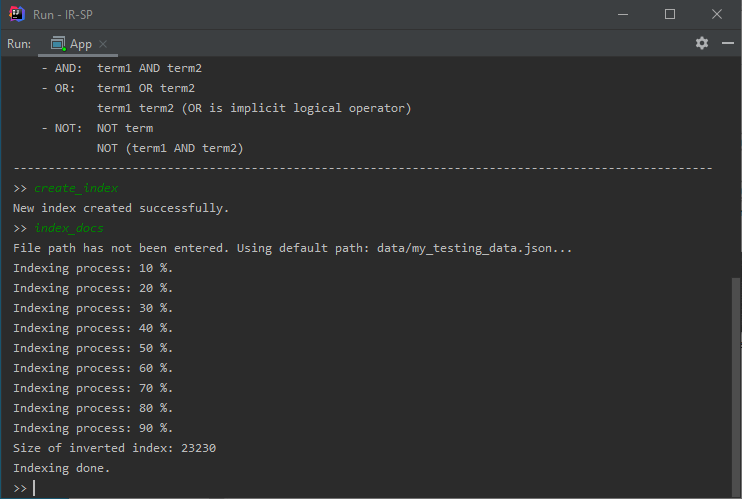
\includegraphics[width=1\textwidth]{img/zaindexovani.png}
	\caption{Zaindexování dokumentů -- defaultní cesta}
	\label{uziv_zaindexovani}
\end{figure}

Aktuálně načtený index lze uložit do souboru příkazem \texttt{save\_index <\textit{název indexu}>}.

\subsection{Vyhledávání v dokumentech}
V dokumentech uložených v aktuálně načteném indexu můžeme vyhledávat dvěma způsoby: 

\begin{enumerate}
    \item příkazem \texttt{search\_normal} -- vyhledá dotaz v zaindexovaných dokumentech prostřednictvím vektorového modelu (toto vyhledávání nepodporuje logické operátory),
    \item příkazem \texttt{search\_boolean} -- vyhledá dotaz v zaindexovaných dokumentech prostřednictvím booleovského modelu (podporuje logické operátory \texttt{AND}, \texttt{OR}, \texttt{NOT}).
\end{enumerate}

Dále je uživatel dotázán na počet nejlepších výsledků, který chce vrátit. Vyhledávání prostřednictvím vektorového modelu je vizualizováno na obrázku \ref{uziv_vyhled}.

\begin{figure}[!ht]
	\centering
	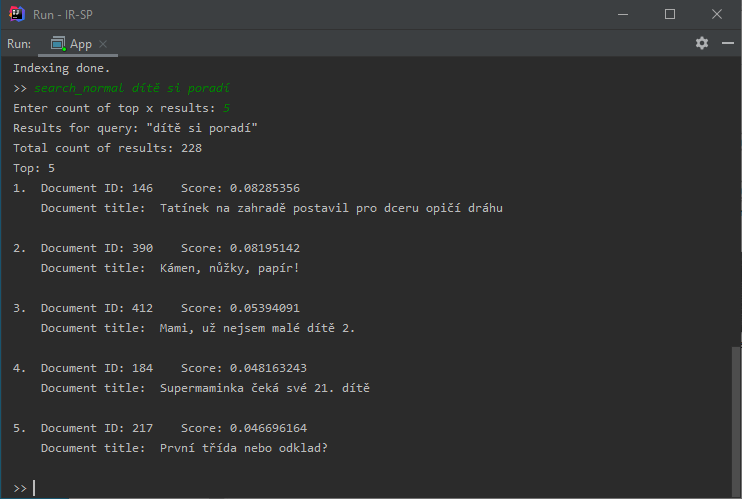
\includegraphics[width=1\textwidth]{img/vyhledavani.png}
	\caption{Vyhledávání prostřednictvím vektorového modelu}
	\label{uziv_vyhled}
\end{figure}

\subsection{Vytvoření, úprava, odstranění dokumentu}\label{CRUD}
V~aktuálně načteném indexu je možné vytvořit nový dokument, upravit existující dokument, či odstranit dokument z indexu. K~tomuto účelu slouží příkazy:

\begin{itemize}
    \item \texttt{create\_doc} -- vytvoří nový dokument v aktuálním indexu (viz obrázek \ref{uziv_vytvor}),
    \item \texttt{update\_doc <\textit{id dokumentu}>} -- upraví existující dokument specifikovaný zadaným id v aktuálním indexu,
    \item \texttt{delete\_doc <\textit{id dokumentu}>} -- odstraní dokument z~aktuálního indexu specifikovaný zadaným id.
    
\end{itemize}

\begin{figure}[!ht]
	\centering
	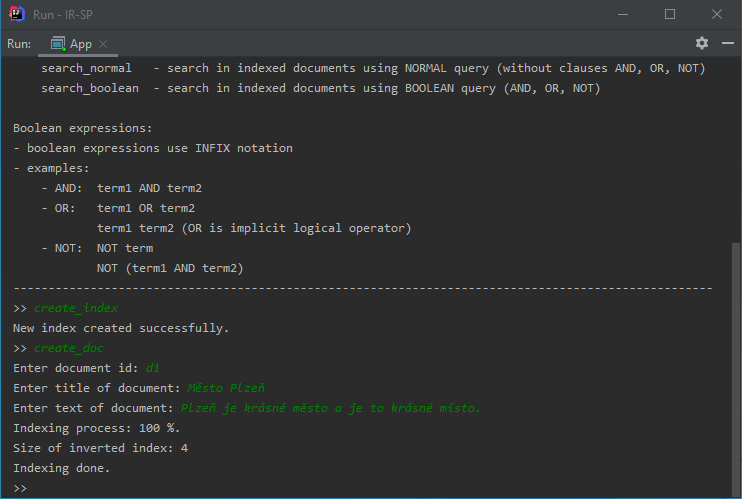
\includegraphics[width=1\textwidth]{img/vytvoreni.png}
	\caption{Vytvoření nového dokumentu v aktuálním indexu}
	\label{uziv_vytvor}
\end{figure}


\chapter{Závěr}
\section{Dosažené výsledky}
Pro různé konfigurace sestavení dotazu vyhledávání jsou výsledky evaluace různé. Záleží, přes která textová pole v evaluačním skriptu \texttt{TestTrecEval} se vyhledává. Vyhledávání je defaultně nastaveno na top $3000$ výsledků. Zde uvádím hodnoty \texttt{map} pro různé konfigurace:

\begin{itemize}
    \item pole \texttt{title} -- $map = 0.1640$,
    \item pole \texttt{description} -- $map = 0.1687$,
    \item pole \texttt{title}, \texttt{description} -- $map = 0.1955$,
    \item pole \texttt{title}, \texttt{description}, \texttt{narrative} -- $map = 0.2378$ (viz výsledky evaluace \ref{vysledky}).
\end{itemize}

\lstset{language=SQL, frame=single, caption={Pole \texttt{title}, \texttt{description} a \texttt{narrative}},  breaklines=true, basicstyle=\small\ttfamily, commentstyle=\itshape, keywordstyle=\bfseries, tab=~, tabsize=2, xleftmargin=5mm, xrightmargin=5mm, label=vysledky}
\renewcommand{\lstlistingname}{Výsledky evaluace}
\begin{lstlisting}
num_q           all     50
num_ret         all     150000
num_rel         all     762
num_rel_ret     all     709
map             all     0.2378
gm_ap           all     0.1053
R-prec          all     0.2478
bpref           all     0.2358
recip_rank      all     0.4186
ircl_prn.0.00   all     0.4654
ircl_prn.0.10   all     0.4192
ircl_prn.0.20   all     0.3616
ircl_prn.0.30   all     0.3116
ircl_prn.0.40   all     0.2934
ircl_prn.0.50   all     0.2621
ircl_prn.0.60   all     0.2205
ircl_prn.0.70   all     0.1809
ircl_prn.0.80   all     0.1416
ircl_prn.0.90   all     0.0867
ircl_prn.1.00   all     0.0646
P5              all     0.2680
P10             all     0.2460
P15             all     0.2240
P20             all     0.1970
P30             all     0.1600
P100            all     0.0778
P200            all     0.0490
P500            all     0.0241
P1000           all     0.0133
\end{lstlisting}

\section{Zhodnocení}
Cílem této semestrální práce bylo implementovat komplexní systém automatické indexace a vyhledávání dokumentů. Realizovaná aplikace je schopná předzpracovat a zaindexovat dokumenty, ve kterých je možné následně vyhledávat prostřednictvím vektorového modelu či booleovského modelu. Vyhledávání prostřednictvím booleovského modelu umožňuje použití logických operátorů AND, OR, NOT a také je možné vynutit prioritu těchto operátorů prostřednictvím závorek.

Minimální funkčnost popsaná v kapitole \ref{min_func} byla splněna. Z~nadstandardního rozšíření (viz kapitola \ref{adv_func}) jsem realizoval file-based index, pozdější doindexování dat, CRUD indexovaných dokumentů a dokumentaci psanou v TEXu. Při implementaci této semestrální práce jsem se nesetkal s většími problémy.\\

\noindent Semestrální práce z mého pohledu splňuje požadavky zadání.

\end{document}